\documentclass{standalone}


\begin{document}

\subsection[Pipeline]{DNetPRO in Snakemake}\label{implementation:snakemake}

The starting (silent) hypothesis done until now is that we are running the \textsf{DNetPRO} algorithm on a single dataset (or better on a single Hold-Out subdivision of our data).
On this configuration it is legal to stress as much as possible the available computational resources and parallel processing each step of the algorithm.

If we want to introduce our algorithm inside a larger pipeline, in which we compare the resulting obtained over a Cross-Validation of our datasets we have to re-think about the parallelization done.
In this case, each fold of the cross validation can be interpreted as an independent task and, following the main programming rule \emph{\quotes{parallelize the outer, vectorize the inner}}, we should spawn a thread for each fold and perform the couple evaluation in sequential mode.
Certainly, the optimal solution would be to separate our jobs across a wide range of inter-connected computers and still perform the same computation in parallel but it would required to implement our hybrid (\textsf{C++} and \textsf{Python}) pipeline in a Message Passing Interface (MPI) environment.

An easier solution to overcome all these problems can raise by the use of \textsf{SnakeMake}~\cite{snakemake} rules.
\textsf{SnakeMake} is an intermediate language between \textsf{Python} and \textsf{Make}.
Its syntax is almost like the \textsf{Make} language, but with the help of the easier and powerful \textsf{Python} functions.
It is widely used for bioinformatic pipeline parallelization since it can easily applied over single or multi-cluster environment (master-slave scheme) with a simple change of command line.

\begin{center}
\begin{figure}[htbp]
\hspace{-2cm}
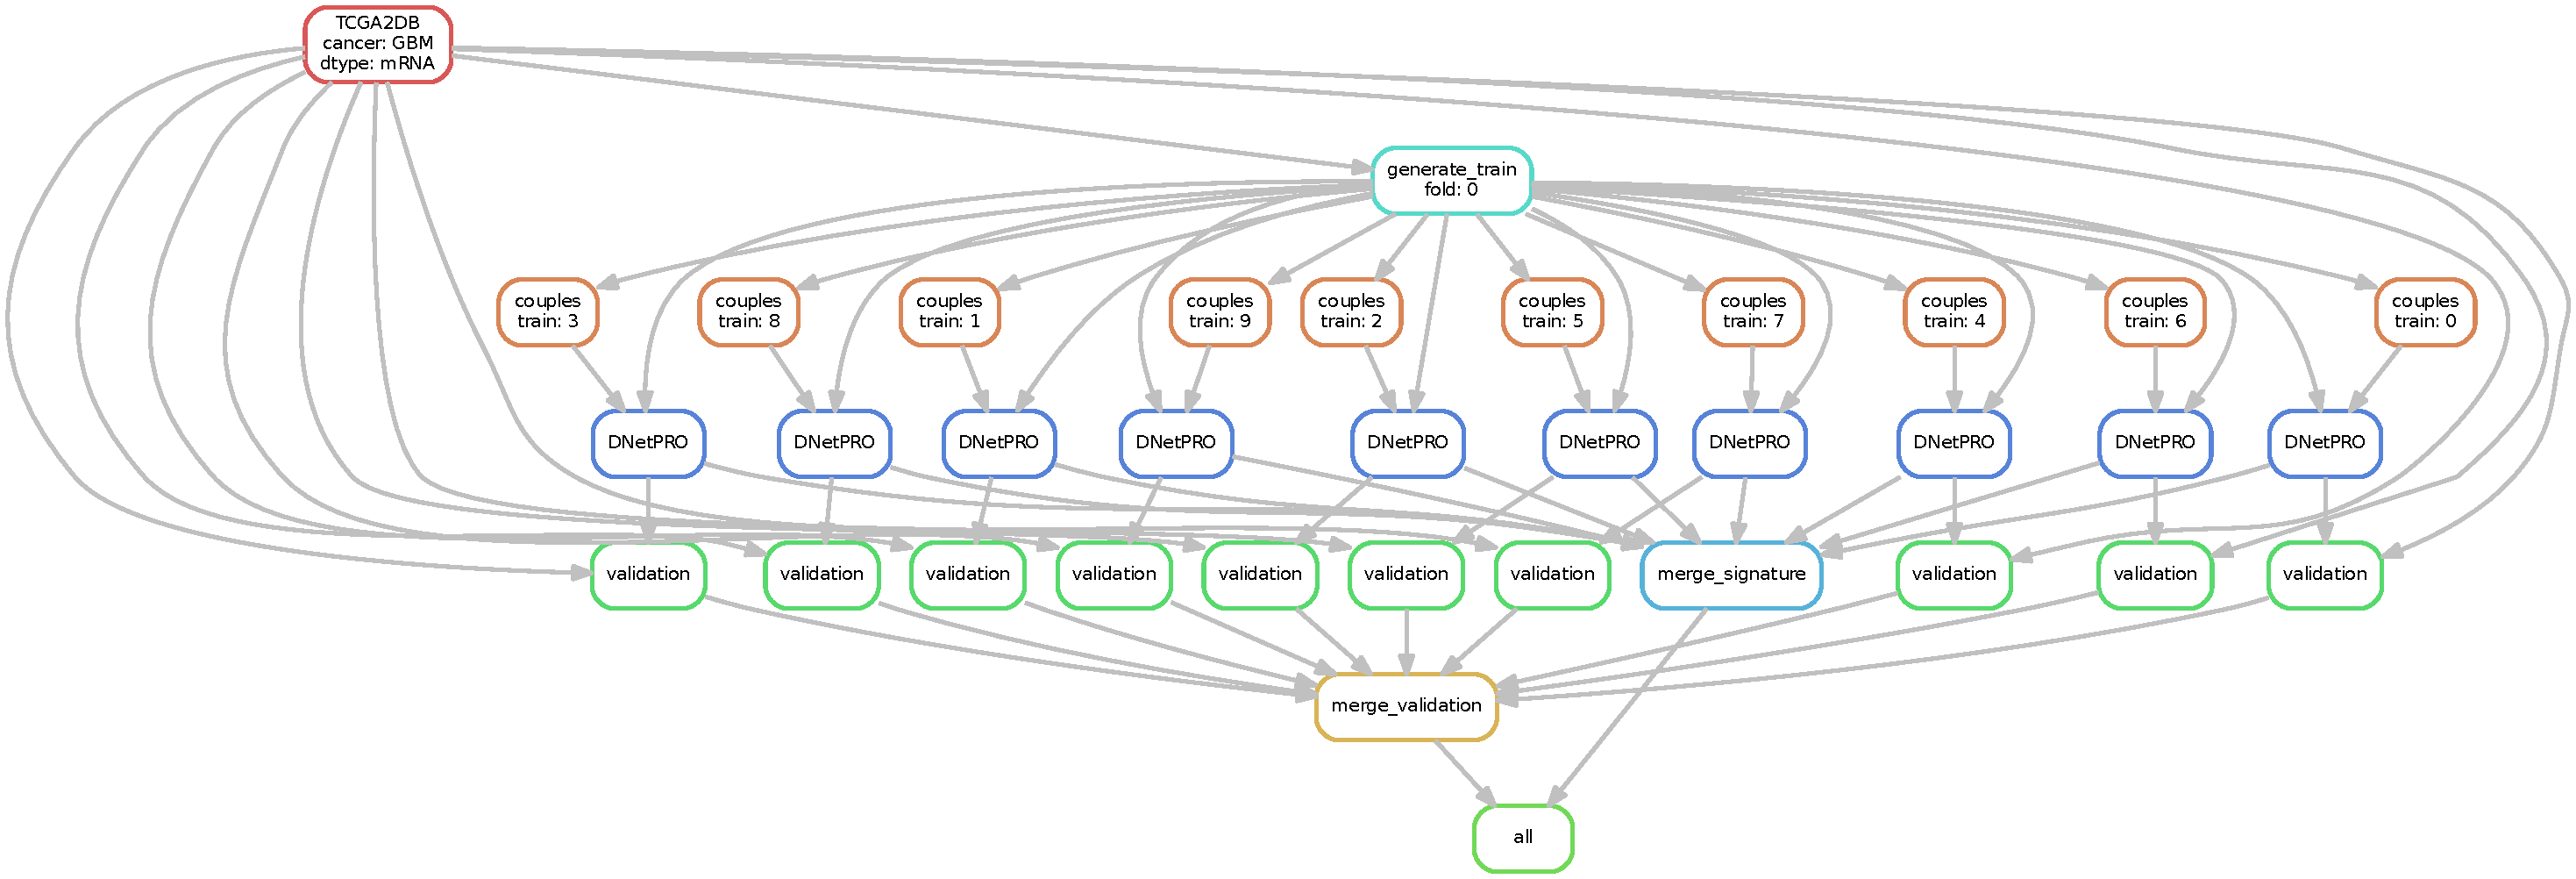
\includegraphics[width=1.3\textwidth]{qdanet_pipe_single.pdf}
\caption{Example of \textsf{DNetPRO} pipeline on a single cross validation.
It is highlighted the independence of each fold from each other.
This scheme shows a possible distribution of the jobs on a multi-threading architecture or for a distributed computing architecture.
The second case allows further parallelization scheme (hidden in the graph) for each internal step (e.g. the evaluation of each pair of genes).
}
\label{fig:dnet_workflow}
\end{figure}
\end{center}

So to improve the scalability of our algorithm we implement the benchmark pipeline scheme using Snakemake rules and a work-flow example for a single cross-validation is shown in Fig.~\ref{fig:dnet_workflow}.
In this case each step of Fig.~\ref{fig:dnet_workflow} can be performed by a different computer unit preserving the multi-threading steps, with a maximum scalability and the possibility to enlarge the problem size and the number of variables.


\end{document}
